\documentclass[12pt,fleqn,x11names,table]{report}                                                  
\usepackage[text={15cm,25cm},centering,headsep=20pt,top=0.8in, bottom = 0.8in,letterpaper,showframe=false]{geometry}
%--------------------------------------------------------------------------
% Paquetes y estilo del libro. http://www.tec-digital.itcr.ac.cr/revistamatematica/
% Versi�n Juio-2014
%--------------------------------------------------------------------------
% Paquetes 
\usepackage[spanish,es-tabla]{babel}
\usepackage[latin1]{inputenc}                   % Entrada de acentos
\usepackage[T1]{fontenc}
\usepackage[autostyle, spanish = mexican]{csquotes}% manejo de comillas: " "
\MakeOuterQuote{"}
\usepackage{pslatex}                              % Fuentes finas postscript
%\usepackage[sc]{mathpazo}                         % Fuentes mathpazo
\usepackage{helvet}
\linespread{1.05}                                  % Fuente Palatino necesita espaciado
\usepackage[full]{textcomp}                        % Caracteres especiales como ' (recto)
\usepackage{xcolor}                                % Color: X11names (en el documentclass)
% COLORES personales---------------------------------------------------
    \definecolor{colortitulo}{RGB}{11,17,79} % 
    \definecolor{colordominante}{RGB}{11,17,79}
    \definecolor{colordominanteA}{RGB}{243,102,25}
    \definecolor{colordominanteF}{RGB}{219,68,14}
    \definecolor{colordominanteD}{RGB}{74,0,148}
   
    \definecolor{wcolornotas}{RGB}{74,0,148}%{RGB}{51,145,147} % 
    \definecolor{mostaza}{RGB}{231,196,25}
    \definecolor{amarilloM}{RGB}{248,199,90}
    \definecolor{amarilloD}{RGB}{251,237,121}
    \definecolor{azulF}{rgb}{.0,.0,.3}
    \definecolor{grisD}{rgb}{.3,.3,.3}
    \definecolor{grisF}{rgb}{.6,.6,.6}
    \definecolor{grisamarillo}{RGB}{248,248,245} 
    \definecolor{miverde}{RGB}{44,162,67}
    \definecolor{verdep}{RGB}{166,206,58}
    \definecolor{verdeF}{RGB}{5,92,8}
    \colorlet{mygray}{black!20}
    \newcommand{\verde}{\color{miverde}}
    \newcommand{\colornotas}{\color{wcolornotas}}
% Fin COLORES personales-------------------------------------------------
\usepackage{psboxit}
\usepackage{pstricks}
\usepackage{xparse}

\usepackage{tikz,tkz-tab}% Cajas de Teoremas, ejemplos, etc.
%listings para c�digo en color en tcbcolor
\usetikzlibrary{matrix,arrows,
positioning,shadows,shadings,backgrounds,calc, shapes, tikzmark}%
\usepackage{tcolorbox, empheq} 
 % Librer�as tcolorbox
\tcbuselibrary{skins,breakable,listings,theorems} 

\usepackage{xargs}                                 % Comandos con opciones
\DeclareGraphicsExtensions{.pdf,.png,.jpg}
\usepackage{multicol}
% %\usepackage{epstopdf}% Conversi�n - Miktes 2.9 o inferior, TexLive 2009. o inferior
\usepackage[small,bf,labelsep=period]{caption}
\usepackage[breaklinks,colorlinks=true, pdfstartview=FitV, linkcolor=azulF, citecolor=azulF, urlcolor=azulF]{hyperref}
\usepackage{amsmath,amssymb,amsfonts,latexsym,cancel,stmaryrd}%
\usepackage[ruled,,vlined,lined,linesnumbered,algochapter]{algorithm2e}
\usepackage{framed}
\usepackage{titletoc}
\usepackage{calc}
\usepackage{longtable} 
\usepackage{colortbl} 
\usepackage{tabularx}
\usepackage{fancyvrb}
%\usepackage{minted}   %habilitar solo en Ubuntu (Linux)
\usepackage{array}
\usepackage{wasysym}
\usepackage{supertabular}
\definecolor{verbmentsbgcolor}{rgb}{0.9764, 0.9764, 0.9762}
\definecolor{verbmentscaptionbgcolor}{rgb}{0.1647, 0.4980, 1}
\usepackage{verbments}
\fvset{frame=bottomline,framerule=0.01cm}
\plset{language=java,texcl=true,style=vs,%
listingnamefont=\sffamily\bfseries\color{white},%
bgcolor=verbmentsbgcolor,captionfont=\sffamily\color{white},%
captionbgcolor=verbmentscaptionbgcolor, listingname=\textbf{Programa}}
%\usepackage{pagecolor}
\usepackage[textwidth=2cm]{todonotes} 
\usepackage{booktabs}
\usepackage{marginnote}
\usepackage[b]{esvect}
\usepackage{rotating}
%\usepackage{float}
\usepackage{floatrow}
\usepackage[shortlabels]{enumitem}
\usepackage{subfigure}
\usepackage{wrapfig}
\usepackage{floatflt}
 \usepackage{kantlipsum} %\kant[1-13]

\renewcommand{\thechapter}{\roman{chapter}}
\renewcommand{\thesection}{\arabic{chapter}.\arabic{section}}
%----------------------------------------------------------------------------------------
% Fuentes especiales
%----------------------------------------------------------------------------------------
% Comandos para fuentes especiales
\newcommandx*{\fnte}[4][1=pag,2=9,3=n]{{\color{azulF}\fontfamily{#1}\fontseries{b}
\fontsize{#2}{1}\fontshape{#3}\selectfont{#4}}}

\newcommandx*{\fntb}[4][1=pag,2=9,3=n]{{\color{azulF}\fontfamily{#1}\fontsize{#2}{1}\fontseries{b}\fontshape{#3}\selectfont{#4}}}

\newcommandx*{\fntg}[4][1=pag,2=9,3=n]{{\color{grisF}\fontfamily{#1}\fontsize{#2}{1}\fontshape{#3}\selectfont{#4}}}

\newcommand{\fhv}[2]{{\fontfamily{pag}\fontsize{#1}{1}\selectfont{#2}}}

\newcommand{\fhvb}[2]{{\fontfamily{pag}\fontseries{b}\fontsize{#1}{1}\selectfont{#2}}}

% fontfamily %n = normal, it =italics
\newcommandx*{\fntl}[4][1=pag,2=10,3=n]{{\colornotas\fontfamily{#1}\fontsize{#2}{1}\fontseries{b}\fontshape{#3}\selectfont{#4}}}

\newcommandx*{\tfntl}[4][1=pag,2=10,3=n]{{\color{azulF}\fontfamily{#1}\fontsize{#2}{1}\fontseries{b}\fontshape{#3}\selectfont{#4}}}

\newcommandx*{\fnt}[4][1=pag,2=9,3=n]{{\colornotas\fontfamily{#1}\fontsize{#2}{1}\fontshape{#3}\selectfont{#4}}}

\newcommandx*{\colrfnt}[4][1=pag,2=9,3=n]{{\red\fontfamily{#1}\fontsize{#2}{1}\fontshape{#3}\selectfont{#4}}}

\newcommandx*{\nfnt}[4][1=pag,2=9,3=n]{{\fontfamily{#1}\fontsize{#2}{1}\fontshape{#3}\selectfont{#4}}}

\newcommand{\wfont}[2]{{\fontfamily{#1}\selectfont{#2}}}
\newcommand{\fptm}[1]{{\fontfamily{ptm}\selectfont{#1}}}

\newcommandx*{\cfnte}[4][1=pag,2=9,3=n]{{\wcelestetxt\fontfamily{#1}\fontsize{#2}{1}\fontshape{#3}\selectfont{#4}}}
% Fin fuentes----------------------------------------------------------

%----------------------------------------------------------------------------------------
% Cabeceras
%----------------------------------------------------------------------------------------
% Elimina el encabezado de las p�ginas impares vac�as al final de los cap�tulos
\makeatletter
\renewcommand{\cleardoublepage}{
\clearpage\ifodd\c@page\else
\hbox{}
\vspace*{\fill}
\thispagestyle{empty}
\newpage
\fi}
%\makeatother

\usepackage{fancyhdr}
% N�meros de p�gina en rect�ngulos y cap�tulo. Necesitamos posicionar los nodos
\usepackage[absolute]{textpos}
    \setlength{\TPHorizModule}{10mm}% 1 generic horizontal unit is equivalent to 10mm
    \setlength{\TPVertModule}{10mm}% 1 generic vertical unit is equivalent to 10mm
    \textblockorigin{0mm}{0mm}% top left corner set as origin

%\makeatletter
% Redefinir \chaptermark sin "cap�tulo" ni n�mero de cap�tulo, solo el texto.
\renewcommand{\chaptermark}[1]{\markboth{\if@mainmatter\ ~~\fi#1}{}}
\makeatother

%------------------------------------------------------------------------------
% Decoraci�n de cabeceras 
% Texto en secciones
\renewcommand{\sectionmark}[1]{\markright{\sffamily\normalsize\thesection\hspace{5pt}#1}{}} 
% Configuraci�n de fuentes para el n�mero de p�gina en el encabezado
\fancyhf{} 
% > OP 1: Todas las p�ginas con la secci�n a la izquierda
%   \fancyhead[LO,LE]{\rightmark} % L=Left, O=Odd y  E=Even pages
% > OP 2: Todas las p�ginas con la seci�n a la izquierda en un rect�ngulo (todo el header)
%   \usepackage{tikzpagenodes}
%   \fancyhead[LO,LE]{\rightmark
%   \begin{textblock}{1}(0,0)
%   \begin{tikzpicture}[remember picture,overlay]
%   \fill[grisamarillo] (current page.north west) 
%     rectangle
%   ([xshift=2pt,yshift=-3pt]current page.east|-current page header area.south east);
%   \end{tikzpicture}
%   \end{textblock}
%   }
% > OP 3: Todas las p�ginas con la seci�n a la izquierda en rect�ngulo bordes difusos
\usepackage{tikzpagenodes}
\usetikzlibrary{decorations.pathmorphing,calc,shadows.blur,shadings}
\pgfmathsetseed{1}

\pgfdeclaredecoration{irregular fractal line}{init}
{
  \state{init}[width=\pgfdecoratedinputsegmentremainingdistance]
  {
    \pgfpathlineto{\pgfpoint{random*\pgfdecoratedinputsegmentremainingdistance}{(random*\pgfdecorationsegmentamplitude-0.02)*\pgfdecoratedinputsegmentremainingdistance}}
    \pgfpathlineto{\pgfpoint{\pgfdecoratedinputsegmentremainingdistance}{0pt}}
  }
}

\tikzset{
   paper/.style={draw=black!10, blur shadow, shade=bilinear interpolation,
                 lower left=black!20, upper left=black!15, upper right=white, lower right=black!10},
   irregular border/.style={decoration={irregular fractal line, amplitude=0.2},
           decorate,
     },
   ragged border/.style={ decoration={random steps, segment length=7mm, amplitude=2mm},
           decorate,
   }
}
%L=Left, Odd Even - Decoraci�n en encabezado aqui entra el encabezado verde con titulo de ref http
\fancyhead[LO,LE]{}

% Fin decoraci�n cabeceras
\renewcommand{\headrulewidth}{0pt}   % Ancho de la l�nea bajo el encabezado
\addtolength{\headheight}{2.5pt}     % Aumente el espacio alrededor de la cabecera 
\renewcommand{\footrulewidth}{0pt}   % Elimina la l�nea en el pie de p�gina
% Estilo para  "pagestyle plain"
\fancypagestyle{plain}{\fancyhead{}\renewcommand{\headrulewidth}{0pt}} 



% N�meros de p�gina+chaptertitle en rect�ngulo en el borde
\fancyfoot[LE]{
\begin{textblock}{3}(21,5)
\begin{tikzpicture}[overlay]
\node[draw=colordominante,
rectangle,minimum width=2cm, minimum height=2cm,
anchor=west,
fill=colordominante,font=\fontsize{25}{1}\sffamily\bfseries,inner sep=2pt,outer sep=2pt] 
at (-1.5cm,0pt){\textcolor{gray!10}{\thepage}};
%cap
\node[right,line width=1pt,rectangle,
fill=grisamarillo,font=\fontsize{35}{1}\sffamily\bfseries,inner sep=20pt,outer sep=60pt,
rotate=-90] at (current page.south west){\textcolor{gray!30}{\leftmark}};  
\end{tikzpicture}
\end{textblock}
}

\fancyfoot[RO]{
\begin{textblock}{3}(18,5)
\begin{tikzpicture}[overlay]
\node[draw=colordominante,rectangle,minimum width=2cm, minimum height=2cm,
anchor=west,
fill=colordominante,font=\fontsize{25}{1}\sffamily\bfseries,inner sep=2pt,outer sep=2pt] 
at (-1.5cm,0pt){\textcolor{gray!10}{\thepage}};
% %cap
% \node[left,line width=1pt,rectangle,
% fill=grisamarillo,font=\fontsize{35}{1}\sffamily\bfseries,inner sep=20pt,outer sep=60pt,
% rotate=90]at (current page.south west){\textcolor{gray!30}{\leftmark}};    
\end{tikzpicture}
\end{textblock}
}
\setlength\headheight{14.5pt} % 
% Fin cabeceras 

%----------------------------------------------------------------------------------------
% Color en los m�rgenes
%----------------------------------------------------------------------------------------
% \pagecolor{grisamarillo}
% \usepackage{eso-pic}
% \pagecolor{grisamarillo}
% \AddToShipoutPictureBG{%
%  \AtTextLowerLeft{\color{grisamarillo}%
%   \rule[-\footskip]{\textwidth}{\dimexpr\textheight+\footskip}}}

% Fin color m�rgenes


%----------------------------------------------------------------------------------------
% Pr�logo
%----------------------------------------------------------------------------------------
\NewDocumentEnvironment{prologo}{O{}}{%
\chapter*{Pr�logo}
\addcontentsline{toc}{schapter}{\addvspace{30pt}\large\sc\bfseries Pr�logo \hfill \color{azulF}  }
\smallskip\smallskip
\begin{minipage}{0.9\textwidth}
 #1}{\end{minipage}}
 

%----------------------------------------------------------------------------------------
% T�tulo
%----------------------------------------------------------------------------------------
\newcommand*{\titulo}[4]{\begingroup%
\raggedleft 
\vspace*{\baselineskip} % Espacio en blanco en la parte superior de la p�gina
{\Large #1}\\[0.167\textheight] % Autor
{\LARGE\bfseries #2}\\[\baselineskip] % pre-t�tulo
{\textcolor{colortitulo}{\Huge #3}}\\[\baselineskip] % T�tulo
{\Large \textit{#4}}\par % Descripci�n adicional

\vfill % Espacio en blanco entre el bloque de t�tulo y "la editorial"

{\raggedright
\begin{minipage}[c]{0.08\textwidth}
\raisebox{-2.0cm}{\includegraphics[width=1.4cm]{images/logo}}
 \end{minipage}
\  \ \hfill\begin{minipage}[t]{0.9\textwidth}
{\color{gray}
 \fhv{9}{Revista digital}\\
 \fhvb{9}{\color{azulF}Matem�tica, Educaci�n e Internet.}
  \fntg[pag][8]{\color{grisF}
  \href{http://www.tec-digital.itcr.ac.cr/revistamatematica/}{(http://www.tec-digital.itcr.ac.cr/revistamatematica/).}}}
\end{minipage}          
}%raggedright
\vspace*{3\baselineskip} % Espacio en blanco antes del final de p�gina
\endgroup}
% Fin Titulo--------------------------------------------------------


%----------------------------------------------------------------------------------------
% Copypright, ISBN, ...
%----------------------------------------------------------------------------------------
\def\copyrightpage{\thispagestyle{empty}%
\vbox to\textheight\bgroup\vfill\obeylines\obeyspaces\xcopyrightpage}

\def\xcopyrightpage#1#2\end#3{\scriptsize\parindent=0pt
Copyright\copyright{#1} 
\vskip40pt
#2\vskip200pt\egroup\endgroup}
\let\endcopyrightpage\relax


%Imprimir info  al pie de p�gina
\makeatletter 
\newif\ifoffprintinfo
\def\dooffprintinfo{\global\offprintinfotrue}

\def\copyrightyear#1{\def\thecopyrightyear{#1}}

\copyrightyear{\the\year}

\def\dofnote#1#2{\vtop{\hyphenpenalty=10000
\advance\hsize -10pt \raggedright
\footnotesize{\it #1. }{ #2}\\
\noindent\hbox{\footnotesize
Derechos Reservados \copyright\ \thecopyrightyear\ Revista digital Matem\'atica, Educaci\'on e Internet
 ({\scriptsize\tt www.tec-digital.itcr.ac.cr/revistamatematica/)}}}}

\def\offprintinfo#1#2{
\def\theoffprint{\bgroup\frenchspacing
\dofnote{#1}{#2}
\egroup}}

\def\x@makefntext#1{
\kern-3\p@
\hrule\@width.4\columnwidth
\kern2.6\p@
\vrule height 9pt width0pt \relax
#1}

\def\offprintinfoerror{\typeout{^^J^^J
!! Debe poner {\string\offprintinfo\string{(Title,
Edition)\string}\string{(Author)\string}^^J en el inicio del documento.!!^^J^^J}}
\bgroup
\x@makefntext{Debe poner {\tt \string\offprintinfo\string{(Title,
Edition)\string}\string{(Author)\string}\newline en el inicio del documento.\vrule depth8pt width0pt}\egroup}}


\def\printoffprintinfo{\vtop to0pt{%
\hsize=\textwidth\footnotesize
\expandafter\ifx\csname theoffprint\endcsname\relax
\offprintinfoerror\else\theoffprint\fi\vskip1sp\vss}}


\def\@xfootnote[#1]{%
  \protected@xdef\@thefnmark{#1}%
  \@footnotemark\@footnotetext}
\makeatother

% Uso: \inforevista{Edici�n de Textos Cient�ficos con LaTeX}{Walter Mora F., Alex Borb�n A.}
\newcommand{\inforevista}{\protect\footnote[ ]{\printoffprintinfo}}


% Fin Copyright

%----------------------------------------------------------------------------------------
% CONTENIDO 
%----------------------------------------------------------------------------------------

%\usepackage{titletoc}
\contentsmargin{0cm}
\titlecontents{chapter}[1pc]
{\addvspace{20pt}%
  \begin{tikzpicture}[remember picture, overlay]%
  \draw[fill=verdep!70,draw=verdep!70] (-4,-.1) rectangle (-0.1,0.5);%
  \pgftext[left,x=-1.5 cm,y=0.2cm]{\color{azulF}\Huge\sc\bfseries \thecontentslabel};%
  \end{tikzpicture}\color{azulF}\large\sc\bfseries%
}%
{}
{}
%{\;\color{verdep!70}\titlerule\;\color{azulF}\large\sc\bfseries P�gina \thecontentspage
{\;\color{verdep!70}\titlerule\;\color{azulF}\large\sc\bfseries \thecontentspage
\begin{tikzpicture}[remember picture, overlay]
\draw[fill=verdep!70,draw=verdep!70] (1pt,0) rectangle (6,0.1pt);
\end{tikzpicture}}%

\titlecontents{section}[2.4pc]
{\addvspace{1pt}}
{\contentslabel[\color{azulF}\thecontentslabel]{2.4pc}}
{}
{\hfill\small \color{azulF}\thecontentspage}
[]
\titlecontents*{subsection}[4pc]
{\addvspace{-1pt}\small}
{}
{}
{\hfill\small \color{azulF}\thecontentspage}
[\\][]

\makeatletter
\renewcommand{\tableofcontents}{%
\chapter*{%
\vspace*{20\p@}%
\begin{tikzpicture}[remember picture, overlay]%
\pgftext[right,x=8cm,y=0.2cm]{\color{azulF}\Huge\sc\bfseries \contentsname};%
\draw[fill=verdep!70,draw=verdep!70] (6,-1) rectangle (20,1.75);%
\clip (6,-1) rectangle (20,1.75);
%\pgftext[right,x=15cm,y=0.2cm]{\color{white}\Huge\sc\bfseries \contentsname};%
\pgftext[right,x=8cm,y=0.2cm]{\color{azulF}\Huge\sc\bfseries \contentsname};%
\end{tikzpicture}}%
\@starttoc{toc}}
\makeatother
% Fin Contenido 






%----------------------------------------------------------------------------------------
% CAPITULO Estilo simple AQUI SE MODIFICA EL CAPITULO
%----------------------------------------------------------------------------------------

\usepackage{titlesec}
\newcommand{\hsp}{\hspace{100pt}}
%\titleformat{\chapter}[hang]{\huge\bfseries}{{
%        \fontsize{6em}{6em}\selectfont\black
%        \thechapter}\hsp\textcolor{verdep}{\vrule height 4em width 2pt}\hsp}{0pt}{\huge%\bfseries}
% Subir el t�tulo
       
%-
\titleformat{\chapter}[display]{\normalfont\LARGE\bfseries}%
{\titlerule[1pt]\vspace{1pt}%
\titlerule
\vspace{1pc}%
\filcenter\textcolor{verdep}{\Huge\MakeUppercase{\chaptertitlename} \thechapter}}
{1pc}
{\titlerule
\vspace{2pc}%
\filcenter\fontsize{6em}{6em}\selectfont\black\LARGE}
%%--



%----------------------------------------------------------------------------------------
%	Numeraci�n de las secciones -- en el margen
%----------------------------------------------------------------------------------------

\makeatletter
\renewcommand{\@seccntformat}[1]{\llap{\textcolor{verdeF}{\csname the#1\endcsname}\hspace{1em}}}                    
\renewcommand{\section}{\@startsection{section}{1}{\z@}
{-4ex \@plus -1ex \@minus -.4ex}
{1ex \@plus.2ex }
{\color{azulF}\normalfont\large\bfseries}}
\renewcommand{\subsection}{\@startsection {subsection}{2}{\z@}
{-3ex \@plus -0.1ex \@minus -.4ex}
{0.5ex \@plus.2ex }
{\normalfont\sffamily\bfseries}}
\renewcommand{\subsubsection}{\@startsection {subsubsection}{3}{\z@}
{-2ex \@plus -0.1ex \@minus -.2ex}
{0.2ex \@plus.2ex }
{\normalfont\small\sffamily\bfseries}}                        
\renewcommand\paragraph{\@startsection{paragraph}{4}{\z@}
{-2ex \@plus-.2ex \@minus .2ex}
{0.1ex}
{\normalfont\small\sffamily\bfseries}}
\makeatother
% Fin numeraci�n secciones



%---------------------------------------------------------------------------------
%  Entornos:  Ejemplo, teorema, proposici�n, lema, lista de ejercicios, 
%             caja interludio, caja simple  
%---------------------------------------------------------------------------------

%  Cajas con el paquete  tcbcolor
%  CONTADORES: ejemplo, definicion, lema, teorema, corolario, proposicion,ejercicio 
\newcounter{tcbteo}[chapter]
\renewcommand{\thetcbteo}{\thechapter.\arabic{tcbteo}}

\newcounter{tcbdefi}[chapter]
\renewcommand{\thetcbdefi}{\thechapter.\arabic{tcbdefi}}

\newcounter{tcblema}[chapter]
\renewcommand{\thetcblema}{\thechapter.\arabic{tcblema}}

\newcounter{tcbcoro}[chapter]
\renewcommand{\thetcbcoro}{\thechapter.\arabic{tcbcoro}}

%  \newcounter{tcbListaEjercicios}[chapter]
%  \renewcommand{\thetcbListaEjercicios}{\thechapter.\arabic{tcbListaEjercicios}}

\newcounter{tcbpropo}[chapter]
\renewcommand{\thetcbpropo}{\thechapter.\arabic{tcbpropo}}

\newlength{\examlen}
\tikzset{
    wnodeTeorema/.style={%
         rectangle,  top color=gray!5, bottom color=gray!5,
         inner sep=1mm,anchor=west,font=\small\bf\sffamily},
   wnodeminimo/.style={%
         rectangle,  top color=white, bottom color=white,
         text=azulF,inner sep=1mm,anchor=west,font=\small\bf\sffamily}      
}



%\begin{teorema}  o \begin{teorema}[de tal] o \begin{teorema}[][ref]
% Teorema -----------------------------------------------------
\newtcolorbox{wwteorema}[3][]{%
arc=0mm,breakable,enhanced,colback=gray!5,boxrule=0pt,top=7mm,
drop fuzzy shadow,
fontupper=\normalsize,step and label={tcbteo}{#3},
% Caso normal, sin quiebres
overlay unbroken ={%
\draw[color=colordominanteD,line width=0.2pt] (frame.north west)--([xshift=0pt]frame.north east);
%Caja de T�tulo: teo --
\node[wnodeTeorema](tituloteo) at ([xshift=0pt, yshift=-4mm]frame.north west)
{\textbf{\color{colordominanteD} Teorema \thetcbteo \;#2}};
%Borde superior --
\draw[colordominanteD,line width=2.5cm] ([xshift=1.25cm, yshift=0cm]frame.north west)-- +(\examlen,3pt);
},
% Caso de quiebre por cambio de p�gina
overlay first = {%
\draw[color=colordominanteD,line width=0.2pt] (frame.north west)--([xshift=0pt]frame.north east);
%Caja de T�tulo: teo --
\node[wnodeTeorema](tituloteo) at ([xshift=0pt, yshift=-4mm]frame.north west)
{\textbf{\color{colordominanteD} Teorema \thetcbteo \;#2}};
%Borde superior --
\draw[colordominanteD,line width=2.5cm] ([xshift=1.25cm, yshift=0cm]frame.north west)-- +(\examlen,3pt);
                }, 
overlay middle={},                
% Mantener borde en cambio de p�gina 
overlay last = {\draw[color=colordominanteD,line width=0.2pt] (frame.north west)--([xshift=0pt]frame.north east);
                } 
#1}
%-
\NewDocumentEnvironment{teorema}{O{} O{} O{}}{\smallskip\begin{wwteorema}{#1}{#2}%
 #3}{\end{wwteorema}\smallskip }
% TEOREMA---------------------------------------------------------



%\begin{proposicion}  o \begin{proposicion}[de tal] o \begin{proposicion}[][ref]
% Proposici�n-----------------------------------------------------
\newtcolorbox{wwpropo}[3][]{%
arc=0mm,breakable,enhanced,colback=gray!5,boxrule=0pt,top=7mm,
fontupper=\normalsize,step and label={tcbpropo}{#3},
% Caso normal, sin quiebres
overlay unbroken ={%
\draw[color=colordominante,line width=0.2pt] (frame.north west)--([xshift=0pt]frame.north east);        
%Caja de T�tulo: propo --
\node[wnodeTeorema](tituloteo) at ([xshift=0pt, yshift=-4mm]frame.north west)
{\textbf{\color{colordominante} Proposici�n \thetcbpropo\;#2}};
%Borde superior --
\draw[colordominante,line width=2.5cm] ([xshift=1.25cm, yshift=0cm]frame.north west)-- +(\examlen,3pt);
%barra vertical
\draw[color=gray,line width=3pt] ([xshift=2pt] frame.north west)--([xshift=2pt] frame.south west);
},
overlay first ={%
\draw[color=colordominante,line width=0.2pt] (frame.north west)--([xshift=0pt]frame.north east);        
%Caja de T�tulo: propo --
\node[wnodeTeorema](tituloteo) at ([xshift=0pt, yshift=-4mm]frame.north west)
{\textbf{\color{colordominante} Proposici�n \thetcbpropo\;#2}};
%Borde superior --
\draw[colordominante,line width=2.5cm] ([xshift=1.25cm, yshift=0cm]frame.north west)-- +(\examlen,3pt);
}, %
overlay middle={%barra vertical
\draw[color=gray,line width=3pt] ([xshift=2pt] frame.north west)--([xshift=2pt] frame.south west);},
% Mantener borde en cambio de p�gina 
overlay last ={\draw[color=colordominante,line width=0.2pt] (frame.north west)--([xshift=0pt]frame.north east);
        }
#1}
%-
\NewDocumentEnvironment{proposicion}{O{} O{} O{}}{\smallskip\begin{wwpropo}{#1}{#2}%
 #3}{\end{wwpropo}\smallskip }
% ---------------------------------------------------------



% LEMA -----------------------------------------------------------
 \newtcolorbox{wwlema}[3][]{%
arc=0mm,breakable,enhanced,colback=gray!5,boxrule=0pt,
top=1mm, left=3pt,
step and label={tcblema}{#3},
fontupper={\small\bf\sffamily {\color{azulF}Lema \thetcblema \;#2}}~\normalfont, %"Lema..."+texto del cuerpo
overlay unbroken ={%
%barra vertical
\draw[color=gray,line width=3pt] ([xshift=2pt] frame.north west)--([xshift=2pt] frame.south west);
},
overlay first  = {%barra vertical
\draw[color=gray,line width=3pt] ([xshift=2pt] frame.north west)--([xshift=2pt] frame.south west);
},     
overlay middle={%barra vertical
\draw[color=gray,line width=3pt] ([xshift=2pt] frame.north west)--([xshift=2pt] frame.south west);}, 
% Mantener borde en cambio de p�gina     
overlay last ={\draw[color=gray,line width=3pt] ([xshift=2pt] frame.north west)--([xshift=2pt] frame.south west);   }    
#1}
%-
\NewDocumentEnvironment{lema}{O{} O{} O{}}{\smallskip\begin{wwlema}{#1}{#2}%
#3}{\end{wwlema}\smallskip }
%LEMA--------------------------------------------------------------


% % Corolario -------------------------------------------------------
\newtcolorbox{wwcoro}[2][]{%
arc=0mm,breakable,enhanced,colback=gray!5,boxrule=0pt,
top=1mm,left=3pt,
fontupper={\small\bf\sffamily {\color{azulF}Corolario \thetcbcoro}\;}~\normalfont, 
step and label={tcbcoro}{#2},
overlay unbroken ={%
%barra vertical
\draw[color=gray,line width=3pt] ([xshift=2pt] frame.north west)--([xshift=2pt] frame.south west);  
},
overlay first  = {%barra vertical
\draw[color=gray,line width=3pt] ([xshift=2pt] frame.north west)--([xshift=2pt] frame.south west);                 
        },%
overlay middle={%barra vertical
\draw[color=gray,line width=3pt] ([xshift=2pt] frame.north west)--([xshift=2pt] frame.south west);},        
% Mantener borde en cambio de p�gina     
overlay last ={\draw[color=gray,line width=3pt] 
                     ([xshift=2pt] frame.north west)--([xshift=2pt] frame.south west);
              }     
#1}
%-
\NewDocumentEnvironment{corolario}{O{} O{}}{\smallskip\begin{wwcoro}{#1}%
}{\end{wwcoro}\smallskip }
% Corolario------------------------------------------------------


% % Definici�n---------------------------------------------------
\newtcolorbox{wwdefinicion}[3][]{%
arc=0mm,breakable,enhanced,colback=gray!5,boxrule=0pt,drop fuzzy shadow,
top=6mm,fontupper=\normalsize,step and label={tcbdefi}{#3},
overlay unbroken ={%
%barra vertical
\draw[color=colordominanteA,line width=3pt] ([xshift=2pt] frame.north west)--([xshift=2pt] frame.south west);                           
%Caja de T�tulo: defi --
%\node[wnodeTeorema](titulodefi) at ([xshift=4.5pt, %yshift=-3mm]frame.north west)
%{\textbf{Definici�n \thetcbdefi \;#2}};
},
overlay first  = {
%barra vertical
\draw[color=colordominanteA,line width=3pt] ([xshift=2pt] frame.north west)--([xshift=2pt] frame.south west);                         
%Caja de T�tulo: defi --
%\node[wnodeTeorema](titulodefi) at ([xshift=4.5pt, %yshift=-3mm]frame.north west)
%{\textbf{Definici�n \thetcbdefi \;#2}};
                }, %overlay
% Mantener borde en cambio de p�gina
overlay middle={%barra vertical
\draw[color=colordominanteA,line width=3pt] ([xshift=2pt] frame.north west)--([xshift=2pt] frame.south west); 
}, 
overlay last    = {%barra vertical
\draw[color=colordominanteA,line width=3pt] ([xshift=2pt] frame.north west)--([xshift=2pt] frame.south west);}
#1}
%-
\NewDocumentEnvironment{definicion}{O{} O{} O{}}{\smallskip\begin{wwdefinicion}{#1}{#2}%
 #3}{\end{wwdefinicion}\smallskip }
% %DEFINICION---------------------------------------------------------


% Caja para Ejemplo --------------------------------------------------
\newcounter{tcbejem}[chapter]
\renewcommand{\thetcbejem}{\thechapter.\arabic{tcbejem}}
\colorlet{colorfondoejemplo}{gray!5}
\definecolor{colorejemplo}{rgb}{.0,.0,.3}
% Ejemplo
\newtcolorbox{wwejemplo}[3][]{%
arc=0mm,
breakable,drop fuzzy shadow,
enhanced,
colback=grisamarillo,
boxrule=0pt,
top=8mm, %Separaci�n vertical - inicia texto
enlarge top by=\baselineskip/2+1mm,
enlarge top at break by=0mm,pad at break=2mm,
fontupper=\normalsize,
step and label={tcbejem}{#3},
overlay unbroken={%barra vertical
\draw[color=verdep,line width=3pt] ([xshift=2pt] frame.north west)--([xshift=2pt] frame.south west);                            
% Caja de imagen Ejemplo
\node[rectangle, 
         text=black, 
         inner sep=1mm,anchor=west,font=\small\bf\sffamily] at ([xshift=-14.3pt,yshift=-4.1mm]frame.north west)%
{\includegraphics{images/nodoejemplo}\raisebox{0.5cm}{}};
% Caja numeraci�n y descripci�n
\node[rectangle, 
 text=black, 
 inner sep=1mm,
 anchor=west,
 font=\normalsize] at ([xshift=1.1cm,yshift=-2.9mm]frame.north west)%
 {\fhvb{10}{\;\thetcbejem \;\;\;#2}}; }, % overlay
overlay first  = {%
%barra vertical
\draw[color=verdep,line width=3pt] ([xshift=2pt] frame.north west)--([xshift=2pt] frame.south west);                            
% Caja de imagen Ejemplo
\node[rectangle, 
         text=black, 
         inner sep=1mm,anchor=west,font=\small\bf\sffamily] at ([xshift=-14.3pt,yshift=-4.1mm]frame.north west)%
{\includegraphics{images/nodoejemplo}\raisebox{0.5cm}{}};
% Caja numeraci�n y descripci�n
\node[rectangle, 
 text=black, 
 inner sep=1mm,
 anchor=west,
 font=\normalsize] at ([xshift=1.1cm,yshift=-2.9mm]frame.north west)%
 {\fhvb{10}{\;\thetcbejem \;\;\;#2}};
 },%overlay first    
%Borde cambio de p�ginas
overlay middle={%barra vertical
\draw[color=verdep,line width=3pt] ([xshift=2pt] frame.north west)--([xshift=2pt] frame.south west); },
overlay last={%barra vertical
\draw[color=verdep,line width=3pt] ([xshift=2pt] frame.north west)--([xshift=2pt] frame.south west); }
#1}
%-
\NewDocumentEnvironment{ejemplo}{O{} O{} O{}}{\smallskip\begin{wwejemplo}{#1}{#2}%
 #3}{\end{wwejemplo}\smallskip }
%EJEMPLO-----------------------------------------------------------------



% CAJA de comentario-----------------------------------------------------
\definecolor{colrnodocaja}{RGB}{44,91,144}
\definecolor{colrfondocaja}{RGB}{241,241,227}
%CAJA de comentario ------------------------------------------------------
\newtcolorbox{wwcaja}[2][]{%
arc=0mm,breakable,drop fuzzy shadow,
enhanced,colback=gray!4,
boxrule=0pt,
top=3mm, %Separaci�n vertical - inicia texto
enlarge top by=\baselineskip/2+1mm,
enlarge top at break by=0mm,pad at break=2mm,
fontupper=\normalsize,
%step and label={tcbca}{#3},
overlay unbroken ={%
\draw[color=gray!2,line width=0.2pt] (frame.north west)
  --([xshift=0pt]frame.north east)
  --([xshift=0pt]frame.south east)
  --([xshift=0pt]frame.south west)--(frame.north west);
% Caja de T�tulo CAJA
%\node[ rectangle, %minimum width=0cm, minimum height=0.0cm,
%         top color=amarilloD, bottom color=amarilloD,
%         inner sep=0.5mm,anchor=west,font=\normalsize]at ([xshift=-0.5pt,  %yshift=2.30mm]frame.north west){\fnte[pag][10]{ \bf #2}};
},
%Borde
overlay first={\draw[color=gray!2,line width=0.2pt] (frame.north west)
  --([xshift=0pt]frame.north east)
  --([xshift=0pt]frame.south east)
  --([xshift=0pt]frame.south west)--(frame.north west);
% Caja de T�tulo CAJA
%\node[ rectangle, %minimum width=0cm, minimum height=0.0cm,
%         top color=amarilloD, bottom color=amarilloD,
%         inner sep=0.5mm,anchor=west,font=\normalsize]at %([xshift=-0.5pt,  yshift=2.30mm]frame.north west){\fnte[pag][10]{ \bf #2}};
         },
overlay middle={},         
%Borde cambio de p�gina
overlay last={\draw[color=gray!2,line width=0.2pt] (frame.north west)
  --([xshift=0pt]frame.north east)
  --([xshift=0pt]frame.south east)
  --([xshift=0pt]frame.south west)--(frame.north west);}
#1}
%-
\NewDocumentEnvironment{caja}{O{} O{}}{\smallskip\begin{wwcaja}{#1}%
 #2}{\end{wwcaja}\smallskip }
% CAJA de comentario

% Fin mis entornos---------------------------------------------------------------


%-----------------------------------------------------------------------------
% TABLAS CON Tikz
%----------------------------------------------------------------------------- 
\usepackage{array}
\usetikzlibrary{calc,fit,shadows,arrows,positioning}
\pgfdeclarelayer{background}
\pgfdeclarelayer{foreground}
\pgfsetlayers{background,main,foreground}
%--
%------------------------------------------------------------------------------
% Data Table
%------------------------------------------------------------------------------
\newsavebox{\dataTableContent} % Box
\newenvironment{dataTable}[1] % \new environment
{%
\begin{lrbox}{\dataTableContent}%
\begin{tabular}{#1}}%
%
{%
\end{tabular}
\end{lrbox}
\begin{tikzpicture}
\node [inner xsep=0pt] (tbl){\usebox{\dataTableContent}};
\begin{pgfonlayer}{background}
% table
\draw[rounded corners=1pt,top color=gray!1,bottom color=gray!30,draw=black]
(tbl.north east) rectangle (tbl.south west);
% top line
\draw[rounded corners=1pt,top color=gray!10!black,bottom color=gray!50!black,draw=black]%
($(tbl.north west)$) rectangle ($(tbl.north east)-(0,1.5\baselineskip)$);
% bottom rule
\draw[rounded corners=0.25pt,fill=gray,draw=black]%
(tbl.south west) rectangle ($(tbl.south east)+(0,0.05)$);
\end{pgfonlayer}
\end{tikzpicture}}
% --

  
 
 %---------------------------------------Matrices iluminadas------------------------
 %\usetikzlibrary{matrix,backgrounds}
\pgfdeclarelayer{wfondo}
\pgfsetlayers{wfondo,background,main}  
\NewDocumentCommand{\iluminar}{O{blue!40} m m}{%
\draw[#1, fill=#1] (#2.north west) rectangle (#3.south east);
}
% Ejemplos de entornos--------------------------------------------------------------




%----------------------------------------------------------------------------------------
%---------------------------------------------------------------------------------
%  C�digo de programas (LaTeX en ese caso) con Listings
%---------------------------------------------------------------------------------
% Listings
\usepackage{listings}% uso: \lstinline|section| y \begin{lstlisting}... \end{lstlisting}
\usepackage[scaled=0.83]{beramono} % para font \ttfamily en lstlisting
\lstset{ %
	      language={[LaTeX]TeX}, % lenguaje
	      basicstyle=\bfseries\ttfamily,
	      keywordstyle=\color{blue},
	      commentstyle=\color{brown},	   
	      backgroundcolor=\color{gray!15},
	      showstringspaces=false,
	      flexiblecolumns=true,
	      stringstyle=\ttfamily\color{blue},
	      extendedchars=true,	     
emph={rm,bf,it,sf,sl,sc,tt,gtrdot,lesseqqgtr,fcolorbox
      },     
emphstyle={\color{blue}\textbf}, % Color de caracteres especiales
literate=%
   *{$}{{{\color{red}\$}}}1
    {$$}{{{\color{red}\$\$}}}1
%No dejar l�neas en blanco
}%fin lst
\newcommand{\wlatex}{\lstinline}


%CODIGO PARA EJEMPLOS-------------------------------------------------------


 % Ejemplo con \def
 \def\minorma(#1,#2,#3){\sqrt{#1^2+#2^2+#3^2}} 
 \def\lanorma#1{\minormaprevia(#1)}
 \def\minormaprevia(#1,#2,#3){\sqrt{#1^2+#2^2+#3^2}} 
 
 %ENTORNO TEOREMA
 %% En el pre�mbulo
\definecolor{colordominanteD}{RGB}{74,0,148}
\newcounter{tcbteorema}[chapter] % Contador
\renewcommand{\thetcbteorema}{\thechapter.\arabic{tcbteo}} % Formato 1.1,1.2,...

% Estilo "nodoTeorema" para nodos
\tikzset{nodoTeorema/.style={%
         rectangle,  top color=gray!5, bottom color=gray!5,
         inner sep=1mm,anchor=west,font=\small\bf\sffamily}
}

 % Caja de entorno
\newtcolorbox{cajaTeorema}[3][]{% 
  % Opciones generales
  arc=0mm,breakable,enhanced,colback=gray!5,boxrule=0pt,top=7mm,
  drop fuzzy shadow, fontupper=\normalsize,
  % label
  step and label={tcbteo}{#3},
overlay unbroken= {%
       % Borde superior grueso
     \draw[colordominanteD,line width=2.5cm] 
     ([xshift=1.25cm, yshift=0cm]frame.north west)--+(0pt,3pt);
       % Borde superior 1
     \draw[color=colordominanteD,line width=0.2pt] 
     (frame.north west)--([xshift=0pt]frame.north east);
       % Caja Teorema-contador
    \node[nodoTeorema](tituloteo) at ([xshift=0.2cm, yshift=-4mm]frame.north west)
    {\textbf{\color{colordominanteD} Teorema \thetcbteo \;#2}};               
},
overlay first = {
       % Borde superior grueso
     \draw[colordominanteD,line width=2.5cm] 
     ([xshift=1.25cm, yshift=0cm]frame.north west)--+(0pt,3pt);
       % Borde superior 1
     \draw[color=colordominanteD,line width=0.2pt] 
     (frame.north west)--([xshift=0pt]frame.north east);
       % Caja Teorema-contador
    \node[nodoTeorema](tituloteo) at ([xshift=0.2cm, yshift=-4mm]frame.north west)
    {\textbf{\color{colordominanteD} Teorema \thetcbteo \;#2}};   
                }, %First
  % Nada que mantener en los cambios de p�gina 
overlay middle = { },
overlay last = { } 
#1}
%- Uso \begin{teorema}...  o \begin{teorema}[de tal] o \begin{teorema}[][ref]
\NewDocumentEnvironment{ejteorema}{O{} O{} O{}}{\bigskip\begin{cajaTeorema}{#1}{#2}%
 #3}{\end{cajaTeorema}\bigskip }
 

 
 % ejem LEMA -----------------------------------------------------------
\newtcolorbox[auto counter,number within=section]{cajalema}[2][]{
arc=0mm,breakable,enhanced,colback=gray!5,boxrule=0pt,
top=1mm, left=3pt,
fontupper={\small\bf\sffamily {\color{red}Lema \thetcbcounter \;#2}}~\normalfont, %"Lema..."+texto del cuerpo
overlay unbroken={%
  % Barra vertical
\draw[color=gray,line width=3pt] ([xshift=2pt] frame.north west)--([xshift=2pt] frame.south west);           
                 },
overlay first  = {%barra vertical
\draw[color=gray,line width=3pt] ([xshift=2pt] frame.north west)--([xshift=2pt] frame.south west);           
                },      
% Mantener borde en cambio de p�gina   
overlay middle ={\draw[color=gray,line width=3pt] ([xshift=2pt] frame.north west)--([xshift=2pt] frame.south west);   
                },
overlay last ={\draw[color=gray,line width=3pt] ([xshift=2pt] frame.north west)--([xshift=2pt] frame.south west);   
              }    
#1}
%-
\NewDocumentEnvironment{ejlema}{O{} O{}}{\smallskip\begin{cajalema}{#1}%
#2}{\end{cajalema}\smallskip }
%LEMA--------------------------------------------------------------
 
 
 %\usepackage{xparse}
\NewDocumentCommand{\mimpage}{ O{0.45} +m O{0.45} +m }{%
  \begin{minipage}{#1\textwidth}
  #2
  \end{minipage}%
  \hfill \begin{minipage}{#3\textwidth}
  #4
  \end{minipage}%
}
 
 \usepackage{varwidth}
 
 \newcommand{\msen}{{\rm sen}}
 
 
 % ENTORNOS SIMPLES    %Para jemplos del libro
 \usepackage{amsthm}
 %% ---1
\newtheorem{unteo}{Teorema}[section]
\newtheorem{unejem}{{Ejemplo}}[section] 
\newtheorem{unadefi}{Definici�n}[chapter]
 %% ---
 
 %%--
 \newtheoremstyle{estiloA} % nombre del estilo
  {}  % espacio  por encima del teorema. 
  {}  % espacio  por debajo del teorema. 
  {}  % fuente para el cuerpo del entorno 
  {}  % sangr�a
  {.} % puntuaci�n despu�s de encabezado
  {}  % espacio despu�s de encabezado 
  {}  % Especifique manualmente el encabezado
  
\newtheoremstyle{estiloB}{}{}{}{} % 
  {\color{azulF}\bfseries} % fuente del encabezado
  {.}         % puntuaci�n
  {\newline}  % espacio despu�s del encabezado
  {\thmname{#1}~\thmnumber{\red #2}\thmnote{~\color{azulF}(#3)}}
  


 \theoremstyle{estiloB}
 \newtheorem{unadefiB}{Definici�n}[chapter]
 
 \newtheorem{unteoB}{Teorema}[section]
 
 
 \definecolor{rojoF}{RGB}{212,0,0}
 \newtheoremstyle{estiloC}{}{}{}{}% 
  {\blue\bfseries}%
  {.}{\newline}%
  {\thmname{#1}~\thmnumber{\color{rojoF} #2}\thmnote{~(#3)}}%
  %-
  \theoremstyle{estiloC}
  \swapnumbers % Intercambiar n�mero-teorema
  \newtheorem{unteoC}{Teorema}
 
 %%--
 
   \newcounter{contaCaja}    % contador
  \setcounter{contaCaja}{1} % contador en 1
  \def\thecontaCaja{\thechapter.\arabic{contaCaja}}% Contador con # c�pitulo
  \newenvironment{otraCaja}[1]{
   \bigskip
    \begin{tcolorbox}[
       blank,breakable,parbox=false,top=5pt,left=5pt,bottom=5pt, right=5pt,       
       overlay unbroken = {% 
       \draw[black,line width=0.5pt] ($(interior.north west)+( 0pt,-5pt)$) |-
                ($(interior.north)     +( 0pt, 4pt)$) -|
                ($(interior.north east)+( 0pt,-5pt)$);
            \node [black,fill=white] at ($(interior.north west)+(40pt, 4pt)$)
                   {\sffamily\bfseries #1  \thecontaCaja};
            \draw[black, line width=0.5pt] 
                ($(interior.south east)+( 0pt,10pt)$) |-
                ($(interior.south)     +( 0pt, 0pt)$) -|
                ($(interior.south west)+( 0pt,10pt)$);
            },
        overlay first={
            \draw[black,line width=0.5pt] ($(interior.north west)+( 0pt,-5pt)$) |-
                ($(interior.north)     +( 0pt, 4pt)$) -|
                ($(interior.north east)+( 0pt,-5pt)$);
            \node [black,fill=white] at ($(interior.north west)+(40pt, 4pt)$) {\sffamily\bfseries #1 \thecontaCaja};
            },
        overlay last={
            \draw[black,line width=0.5pt] ($(interior.south east)+( 0pt,10pt)$) |-
                ($(interior.south)     +( 0pt, 0pt)$) -|
                ($(interior.south west)+( 0pt,10pt)$);},
        ]
}{
    \end{tcolorbox}
    \bigskip
}


\newcounter{contaCajaB}    % contador
  \setcounter{contaCajaB}{1} % contador en 1
  \newenvironment{otraCajaB}[1]{
    \begin{tcolorbox}[%
       blank,breakable,parbox=false,top=6mm,left=5pt,bottom=5pt, right=5pt,      
       overlay unbroken = {% 
       \draw[draw=blue!15!white,line width=6mm] ($(interior.north west)+( 0pt,0pt)$) |-
                ($(interior.north)     +( 0pt, 0pt)$) -|
                ($(interior.north east)+( 0pt,0pt)$);
            \node [black,fill=white] at ($(interior.north west)+(40pt, 4pt)$)
                   {\sffamily\bfseries #1  \thecontaCajaB};
            \draw[draw=blue!15!white, line width=0.2mm] 
                ($(interior.south east)+( 0pt,10pt)$) |-
                ($(interior.south)     +( 0pt, 0pt)$) -|
                ($(interior.south west)+( 0pt,10pt)$);
            },
        overlay first={             
       \draw[draw=blue!15!white,line width=6mm] ($(interior.north west)+( 0pt,0pt)$) |-
                ($(interior.north)     +( 0pt, 0pt)$) -|
                ($(interior.north east)+( 0pt,0pt)$);
            \node [black,fill=white] at ($(interior.north west)+(40pt, 4pt)$)
                   {\sffamily\bfseries #1  \thecontaCajaB};
            },
        overlay last={
            \draw[draw=blue!15!white,line width=0.5pt] ($(interior.south east)+( 0pt,10pt)$) |-
                ($(interior.south)     +( 0pt, 0pt)$) -|
                ($(interior.south west)+( 0pt,10pt)$);},
                  ]%tcolorbox
}{
    \end{tcolorbox}
    \bigskip
}
%------------------- 
 
 
 
 
 
 
 
 
 
 





%==============config global==============
\renewcommand{\tablename}{Tabla}
\definecolor{styrmitcrwcgray1}{rgb}{0.2,0.2,0.2}
\definecolor{wcgray}{rgb}{0,0.1333,0.3333}
\usetikzlibrary{arrows}
\usepackage{makeidx}
\makeindex
\usepackage{fourier}
\usepackage{pdfpages}
\usepackage{graphicx}
\DeclareGraphicsExtensions {.jpg,.pdf,.png}
\graphicspath{ {./img/} }
%ITEM DE NUMERACION
\newcommand*{\itembolasazules}[1]{% bolas 3D
\footnotesize\protect\tikz[baseline=-3pt]%
\protect\node[scale=0.68, circle, shade, ball
color=green]{\color{azulF}\Large\bf#1};}

\newcommand*{\itembolas}[1]{% bolas 3D
\footnotesize\protect\tikz[baseline=-3pt]%
\protect\node[scale=0.67, circle, shade, ball
color=azulF]{\color{azulF}\Large\bf#1};}
%================================================
\begin{document}

\pagenumbering{arabic} 
\parindent=0mm    % Sin sangría
\pagestyle{fancy} %decoracion de cabecera numero de pagina
%------------------------------------------------------------------------
%CARÁTULA
%==========================================================
\thispagestyle{empty} %para q no este enumerado la pagina
\begin{center}

{\large\textbf{UNIVERSIDAD NACIONAL DE SAN CRIST�BAL DE HUAMANGA}}


{\large\textbf{FACULTAD DE INGENIER�A DE MINAS, GEOLOG�A Y CIVIL}}


{\large\textbf{ESCUELA PROFESIONAL DE INGENIER�A DE SISTEMAS}}

\end{center}

\begin{center}

\includegraphics[scale=0.49]{unsch}   
\end{center}

\begin{center}
\Large\textbf{\color{colordominanteD} INFORME DE LABORATORIO N� 04 }
\end{center}
\begin{center}
\large{\color{azulF} "REDES LAN VIRTUALES - VLAN" }
\end{center}

\textbf{Docente :} 

  
\hspace{3cm} {\blue Prof. Jos� El�as Yauri Vidalon\\ }

\textbf{Curso     :}

  
\hspace{3cm} {\blue REDES DE COMPUTADORAS [IS-441]\\}

\textbf{Alumno   :  }

\hspace{3cm} {\blue  PARIONA VILCA, Jhon Wilder.\\}

\begin{center}
\begin{Large}
\textbf{\emph{ \underline{Ayacucho - Per�}\\
2019}}
\end{Large}
\end{center}

%=========FIN CARATULA==================================
%==============================================================================  
%	Tabla de contenidos
%--------------------------------------------------------------------------------
\tableofcontents
%====fin tabla de contenido==========

%OBJETIVOS
%==========================================================
\chapter{OBJETIVOS}

\begin{caja}[]
\begin{enumerate}[label=\itembolasazules{}]
\item Implementar redes LAN conmutadas utilizando Cisco Packet Tracer (PT).
\item Observar y reflexionar sobre diferentes implementaciones conectadas utilizando conmutadores: switches y hubs.
\end{enumerate}
\end{caja}
%=========FIN objetivos=========

%marcoConceptual
%==========================================================
  
\chapter{MARCO CONCEPTUAL}

%=====================================
\section{REDES DE \'AREA LOCAL (LAN)}
En el libro de Tanenbaum hace referencia a una clasificaci\'on basada en la distancia y con un ejemplo mas del mundo real.
\begin{caja}[]{
 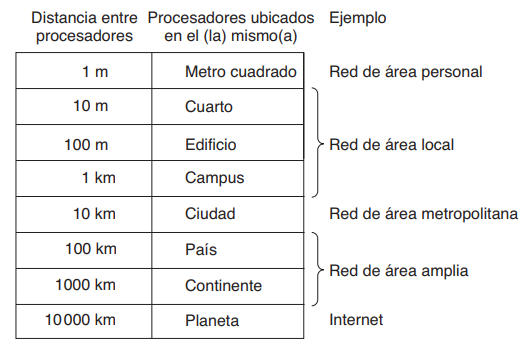
\includegraphics[scale=0.70]{clasifred}
 }\end{caja}
 Seg\'un el gr\'afico una red lan comprender\'ia un cuarto, edificio o campus. Adem\'as Tanenbaum nos menciona que estas redes son de propiedad privada y son utilizadas ampliamente para compartir recursos e intercambiar informaci\'on.\\
 Cuando las empresas usan las redes lan se les conoce como REDES EMPRESARIALES.

Mayormente en los hogares se opta por las conexi\'ones inalambricas

\begin{caja}[]{
 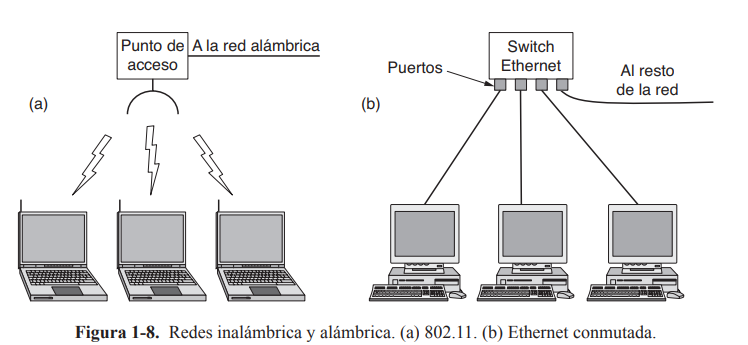
\includegraphics[scale=0.50]{CONEC}
 }\end{caja}
 
Existe un est\'andar para las redes LAN inal\'ambricas llamado IEEE 802.11, mejor conocido como WiFi que opera a velocidades desde 11 hasta cientos de Mbps.
\\
Mientras que para las redes al\'ambrica existe el est\'andar IEEE 802.3, com\'unmente conocido como Ethernet

\\

\begin{definicion}[]
{
Para crear redes LAN m\'as grandes se pueden conectar switches entre s\'i mediante sus puertos.
}
\end{definicion}}
%=====================================0

%========================================
\section{SWICH O CONNMUTADOR}
El trabajo del switch es transmitir paquetes entre las computadoras conectadas a \'el, y utiliza la direcci\'on en cada paquete para determinar a qu\'e computadora se lo
debe enviar. 

%==============================================0

%==============================================
\section{DIRECCI\'ON F\'ISICA MAC (Media Access Control)}
Es un identificador \'unico, son llamadas tambi\'en \textbf{burned-in addresses} ya que son escritas directamente y en forma binaria al momento de la fabricaci\'on del dispositivo.

\begin{definicion}[]
{
Es un identificador de 48 bits donde los primeros  24 bits corresponden al fabricante y los \'ultimos 24 bits es regulada por la IEEE.
\\
la IEEE maneja 3 identificadores globales \'unicos \textbf{MAC-48, EUI-48, y EUI-64}

\end{definicion}}

\begin{caja}[]{
 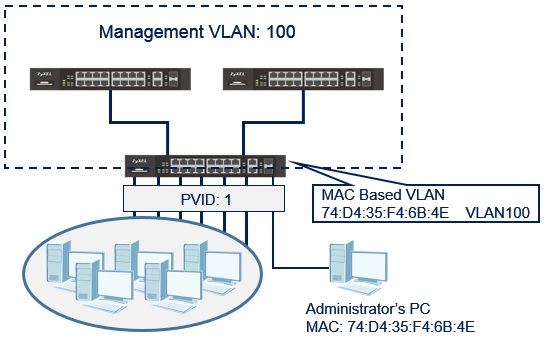
\includegraphics[scale=0.68]{mac}
 }\end{caja}

%==============================================0



\section{HUB O CONCENTRADOR}

\parbox{4cm}{
\begin{caja}[]{
 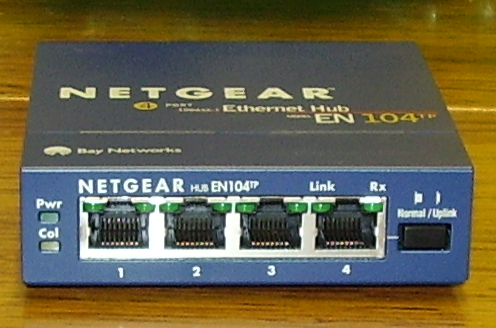
\includegraphics[scale=0.80]{hub}
 }\end{caja}
 } \parbox{10.8cm}{ 
\begin{definicion}[]
{
Trabaja en la capa f\'isica (capa 1) del modelo OSI o la capa de acceso al medio en el modelo TCP/IP. 
\\
Recibe una se\~nal y la repite por sus diferentes puertos.
\\
Actualmente la tarea de los concentradores lo realizan los conmutadores y son m\'as baratos; por ello, los hubs son dificiles de encontrar.
}
\end{definicion}}
\\

%=========FIN objetivos=========

%procedimiento
%==========================================================
\chapter{PROCEDIMIENTO}

\section{Red de Pares: Computador-Computador}

\begin{caja}[]{
 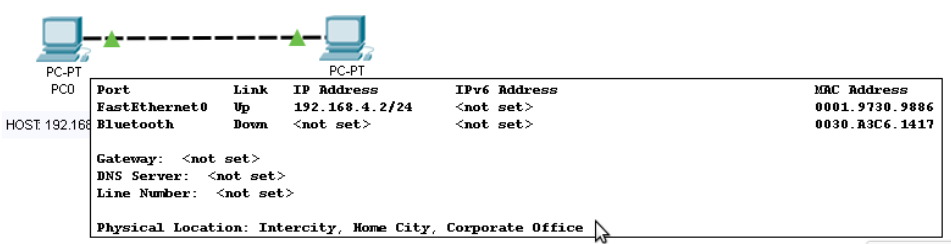
\includegraphics[scale=0.43]{conputador} }
 \end{caja}
 
\begin{definicion}[]{
La configuraci\'on de este tipo de conexi\'on es sencillo; lo \'unico que debemos de hacer es establecer las direcci\'ones ip de cada host.}
\end{definicion}


\subsection{Simule el env\'io de un PDU entre los dispositivos a fin de verificar la conectividad.}
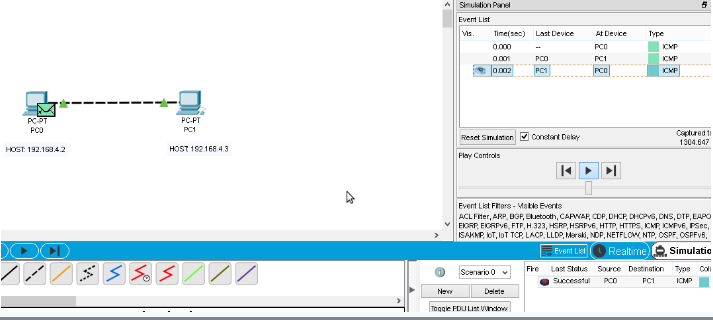
\includegraphics[scale=0.5]{a1}
\begin{definicion}[]{
 vemos que el env\'io es de manera directa entre cada computador
}
\end{definicion}

\subsection{Verifique la conectividad utilizando ping desde la l\'inea de comandos. Repita lo mismo entrando al modo de simulaci\'on.}
Entramos a desktop > command prompt > realizamos el ping
\\
\\
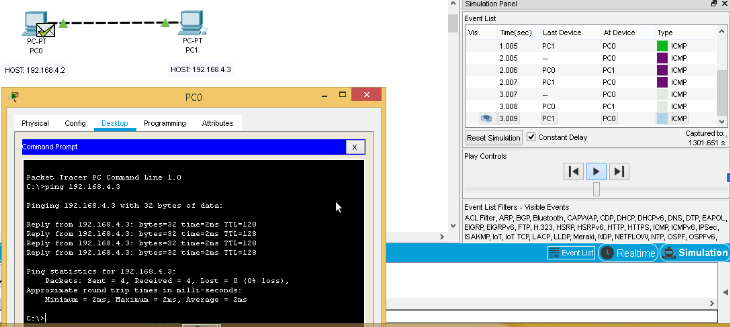
\includegraphics[scale=0.6]{ping}
\begin{definicion}[]
{
 vemos que entre las dos m\'aquinas hay comunicaci\'on de manera correcta.
}
\end{definicion}

\section{Red LAN: Un hub y 04 computadores}
\begin{caja}[]{
 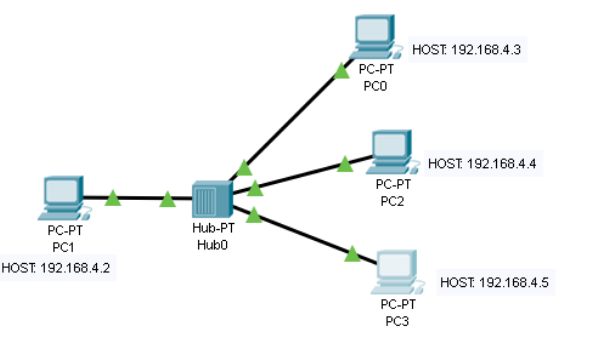
\includegraphics[scale=0.5]{2a} }
 \end{caja}
 
 
 \subsection{Simule el env\'io de un PDU entre la PC0 y PC2. Tome nota del comportamiento del hub.}
 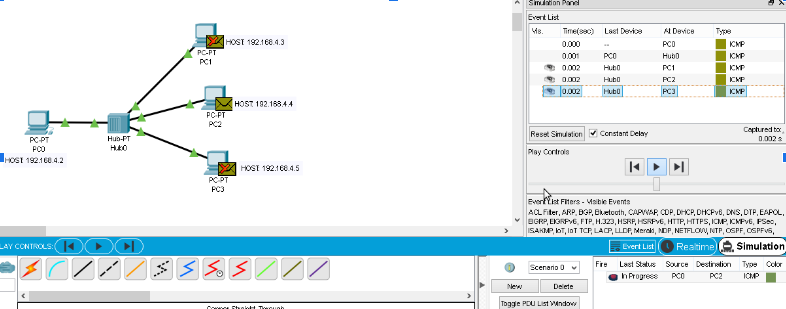
\includegraphics[scale=0.5]{hubpdu}
\begin{definicion}[]
{
 Se puede observar que el paquete viaja a todos los pcs y no solo a al computador destino; pero solo es tomado por el computador destino. Esto podr\'ia ser inseguro ya que todas las computadoras podr\'ian tener acceso al paquete.
}
\end{definicion}


 \subsection{Simule la ejecuci\'on del comando tracert (traceroute). Qu\'e diferencia observa en relaci\'on a la simulaci\'on de con ping}
 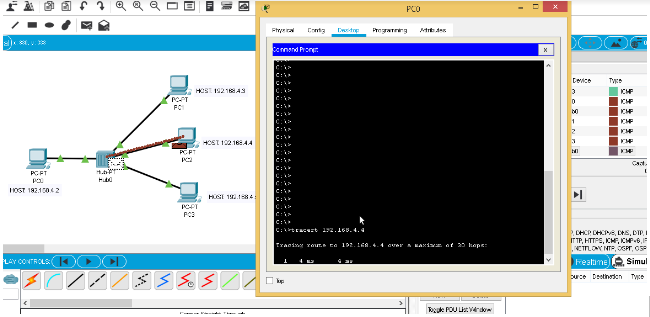
\includegraphics[scale=0.6]{tracert}
\begin{definicion}[]
{
 Al hacer el tracert se observa que demora m\'as y este comando te muestra el m\'inimo tiempo en que llega el paquete y el m\'aximo tiempo.
}
\end{definicion} 


\section{EJERCICIO 1}
\begin{definicion}[]{
Cree una red LAN con dos segmentos de red, donde cada segmento
de red tenga 01 hub y 04 computadoras y est\'en interconectadas
de hub a hub.
}
\end{definicion}

\begin{caja}{
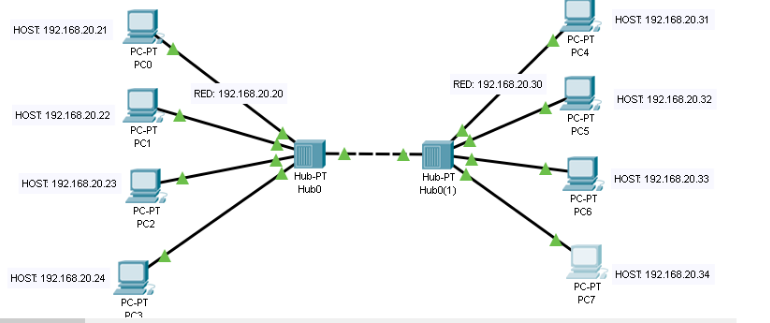
\includegraphics[scale=0.5]{ejercicio1}
}
\end{caja}

\subsection{Compruebe la ejecuci\'on de ping y tracert entre dos dispositivos del mismo segmento y dos dispositivos de segmentos diferentes.}
\subsubsection{Mismo segmento}
	\begin{enumerate}[label=\itembolasazules{}]
\item PING
\\
 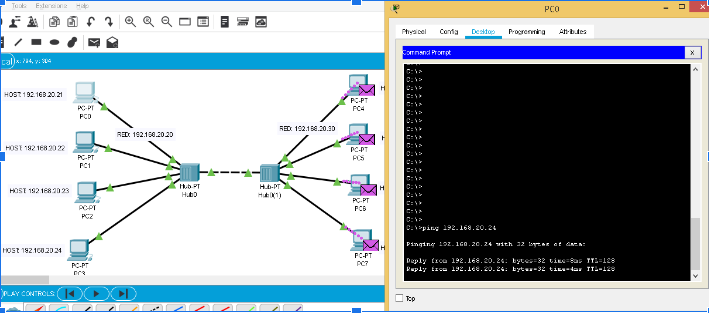
\includegraphics[scale=0.6]{ping1}
\begin{definicion}[]
{
Se puede observar que si hay comunicaci\'on entre la PC0 y la PC3, pero los paquetes tambi\'en llegan al otro segmento del hub.
}
\end{definicion} 
\item TRACERT
\\
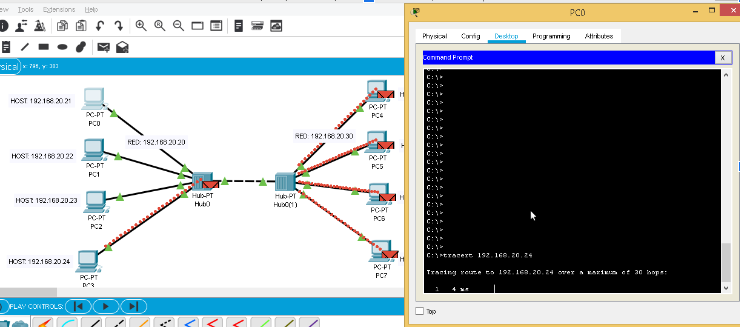
\includegraphics[scale=0.6]{tracert1}
\begin{definicion}[]
{
Se puede observar que la comunnicaci\'on demora mucho m\'as, ya que los paquetes tambi\'en viajan al otro segmento del hub.
}
\end{definicion} 
\end{enumerate}

\subsubsection{Segmentos diferentes}

\begin{enumerate}[label=\itembolasazules{}]
\item PING
\\
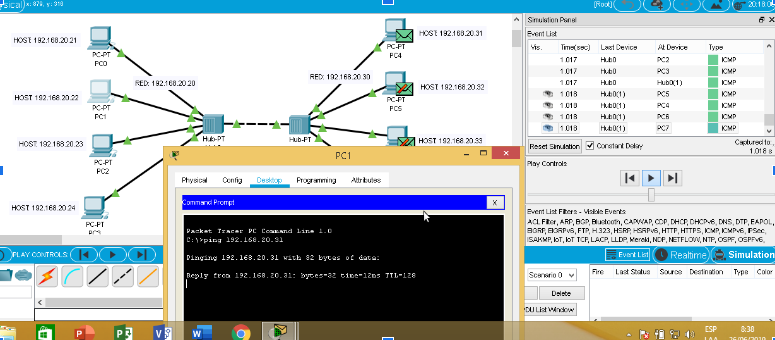
\includegraphics[scale=0.6]{ping2}
\begin{definicion}[]
{
se observa que si hay comunicaci\'on de un segmento a otro(PC1 A PC4).
}
\end{definicion} 
\end{enumerate}
\item TRACERT
\\
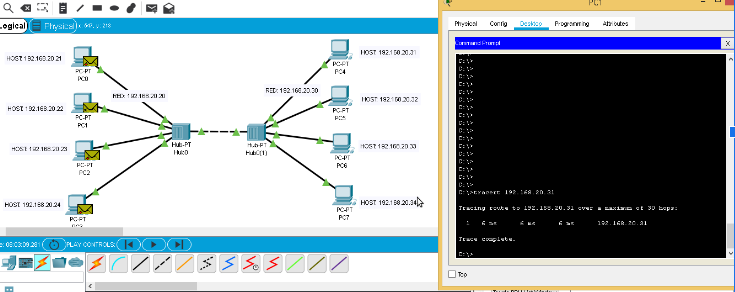
\includegraphics[scale=0.6]{tracert2}
\begin{definicion}[]
{
se observa que si que ahora se demora mucho m\'as).
}
\end{definicion} 
\end{enumerate}

\section{Simule el env\'io de paquetes entre dos hosts del mismo segmento y entre dos hosts de segmentos diferentes.}
\subsubsection{Mismo segmento}
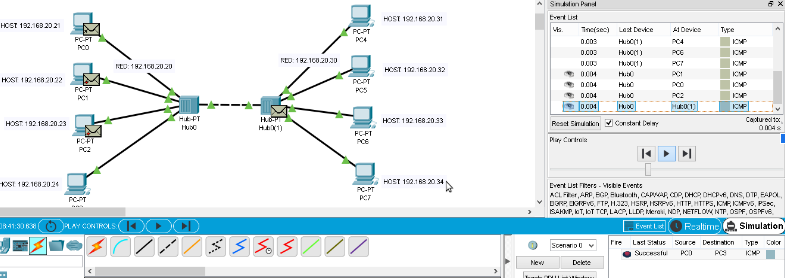
\includegraphics[scale=0.6]{pdu1}
\begin{definicion}[]
{
se observa que el paquete viaja a trav\'es de ambos hubs y llega a todas las m\'aquinas independientemente a quien estemos envi\'andolo
}
\end{definicion} 


\subsubsection{Segmentos diferentes}
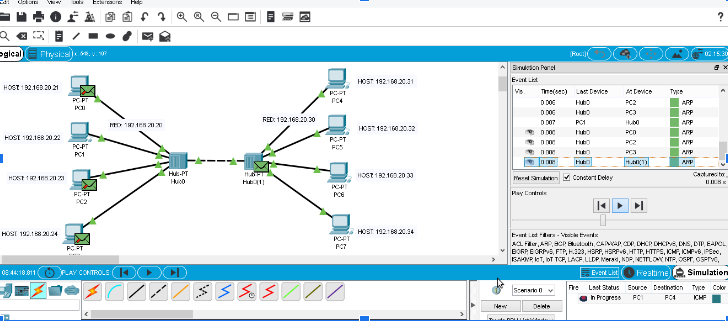
\includegraphics[scale=0.6]{pdu2}
\begin{definicion}[]
{
Al igual que el env\'io anterior el paquete viaja a trav\'es de ambos hubs y llega a todas las PC
}
\end{definicion} 

\subsection{Determine el dominio de colisi\'on}
\begin{definicion}[]
{
El dominio de colisi\'on en este caso ser\'ia toda la red ya que un hub lo que hace difundir el dominio de colisi\'on y no romper el dominio de colisi\'on como si lo hace un conmutador.
}
\end{definicion} 


\section{EJERCICIO 2}
%imagen
\begin{definicion}[]
{
Cree una red LAN con dos segmentos de red, donde un segmento
de red tenga 01 hub y 04 computadoras, mientras que el otro
tenga 04 computadores y est\'en interconectados a un switch. Los
segmentos de red, a su vez, est\'en interconectadas de hub a
switch.\\\\
Como direcciones IP, utilice el rango comprendido entre
192.160.10.50 y 192.160.10.60
}
\end{definicion} 
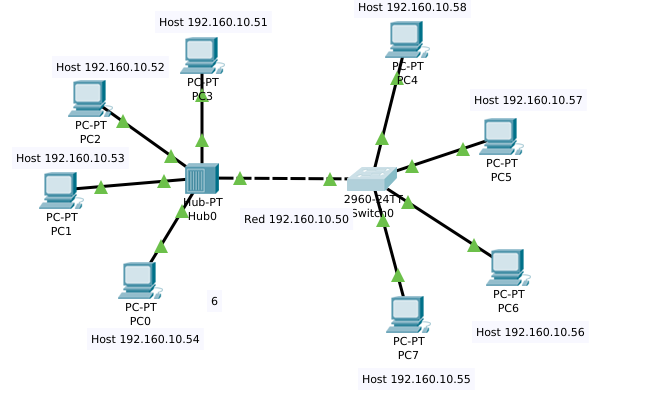
\includegraphics[scale=0.5]{img/dosswitchs.png}
\\\begin{center}
La construcci\'on de la red seria asi.
\end{center}
\subsubsection{Compruebe la ejecuci\'on de ping y tracert entre los distintos nodos de red, adem\'as de simular el env\'io de paquetes simples y complejos entre los distintos nodos.}
\textit{simulamos que todos los nodos se conectan correctamente:}\\

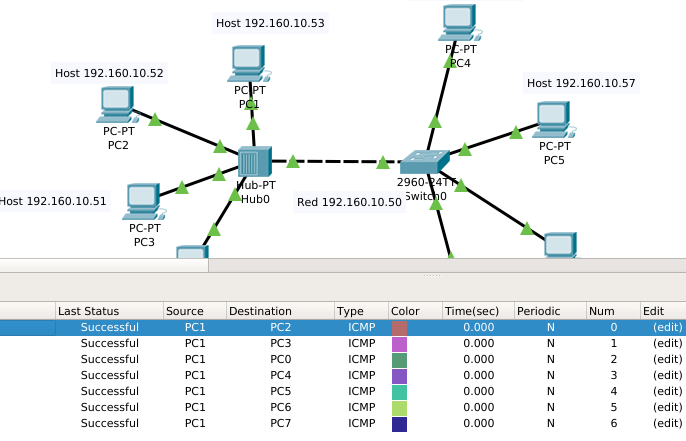
\includegraphics[scale=0.5]{img/prueba1.png} \\
%imagen
%descripcion
\subsubsection{Simule el env\'io de paquetes entre dos hosts del mismo segmento y entre dos hosts de segmentos diferentes.}
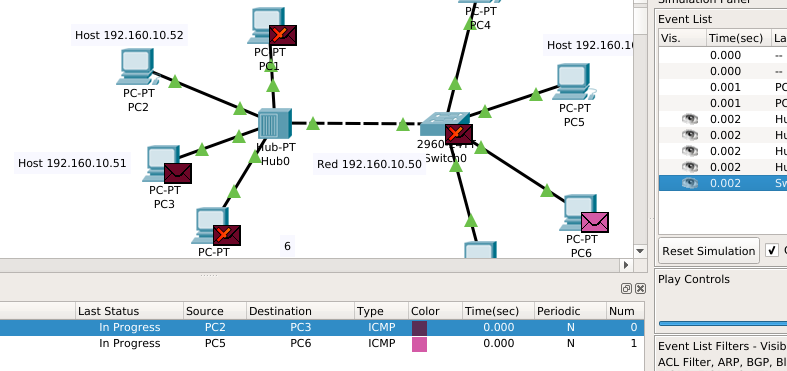
\includegraphics[scale=0.5]{img/simulacion1.png} \\
Como se puede observar el comportamiendo del hub es enviar los paquetes a todos, mientras que el switch no realiza esta acci\'on\\
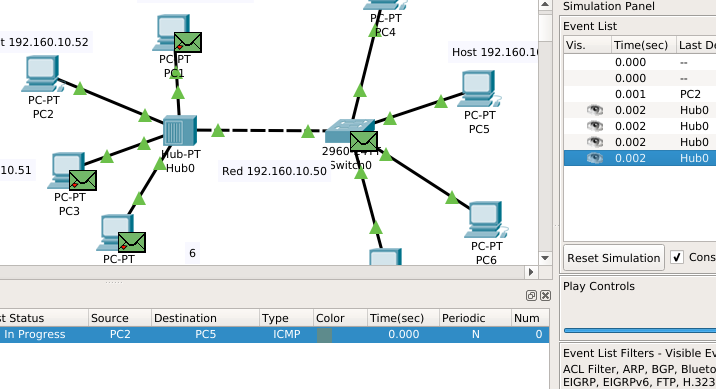
\includegraphics[scale=0.5]{img/simulacion2.png} \\
Para el caso de diferentes segmentos lo que hace el hub es lo mismo que lo anterior.
%imagen
%descripcion
\subsubsection{Determine el dominio de colisi\'on.}
En total hay 5 dominios de colisi\'on ya que un conmmutador rompe el dominio de colisi\'on.
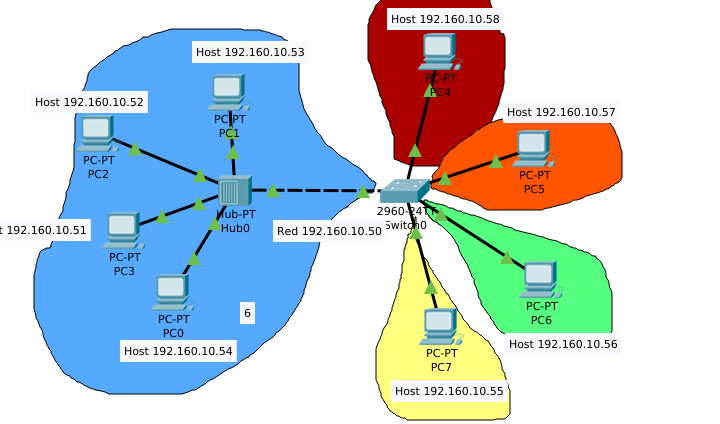
\includegraphics[scale=0.6]{img/dominio.png} 


\section{Red LAN: Switch y 03 Servidores}
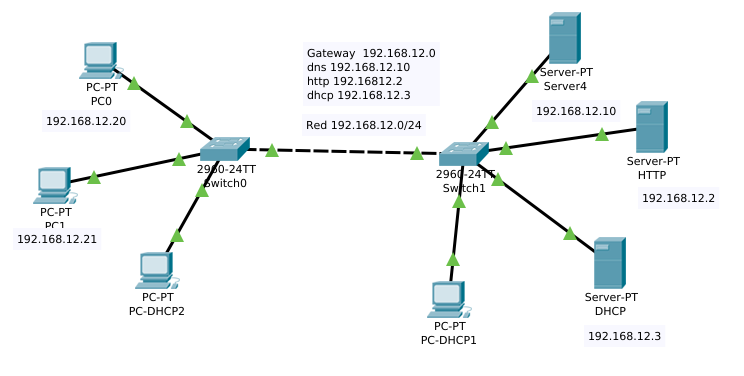
\includegraphics[scale=0.45]{img/switch3ser.png} 
\begin{definicion}[]
{
Hacer ping desde cada una de las PCs al servidor HTTP y
probar el acceso a una p\'agina web dise\~nada por su persona.
}
\end{definicion} 
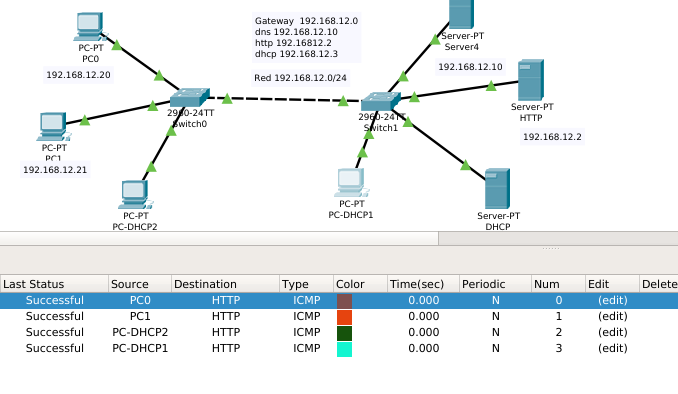
\includegraphics[scale=0.5]{img/pinghttp.png} \\
En este caso lo que hacemos es mandar paquetes para ver si hay conexi\'on por lo que observamos la conexi\'on a sido exitosa.
\\probando que el servidor http funcione\\
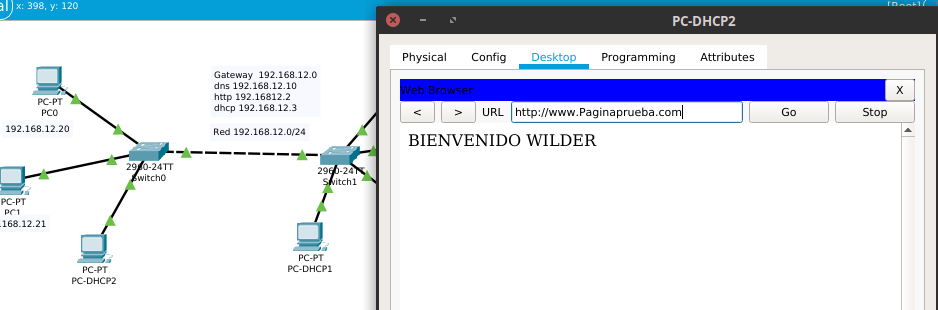
\includegraphics[scale=0.5]{img/prueba.png} \\
el servidor http esta respondiendo de manera adecuada.\\
las configuraciones que hicimos fueron:\\
\textbf{dns}\\
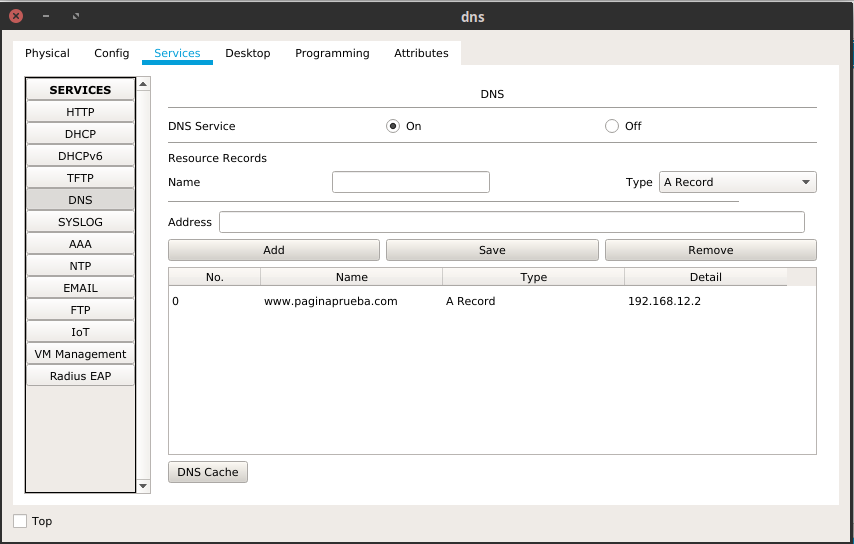
\includegraphics[scale=0.5]{img/dns.png} 
\\En el servidor dns establecemos como ah de llamarse nuestra web a mostrar.\\
\textbf{http}\\
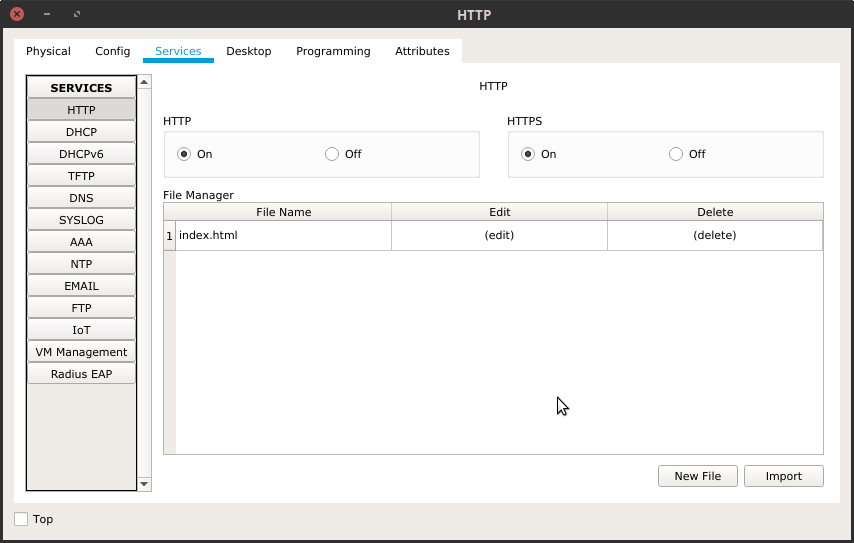
\includegraphics[scale=0.5]{img/http.png}
\\En este servidor configuramos la pagina a mostrar\\
\textbf{dhcp}\\
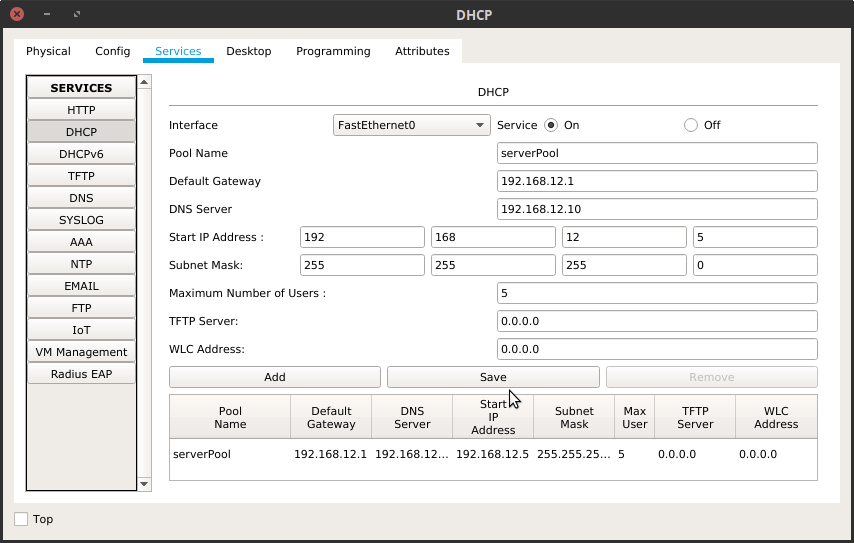
\includegraphics[scale=0.5]{img/dhcp.png} 
\\En este servidor configuramos la ip dinamica que van a recibir las pcs
\\
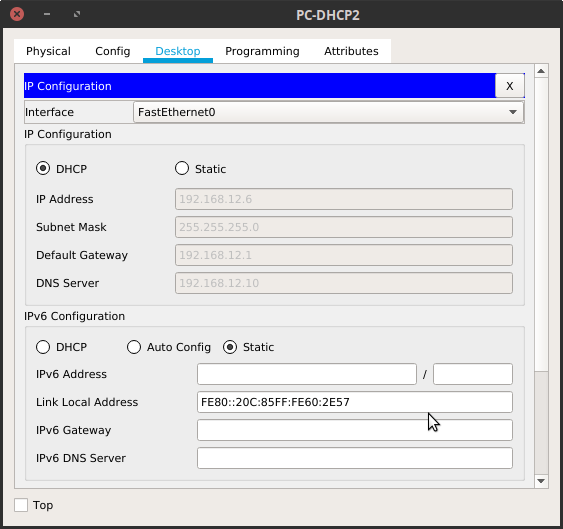
\includegraphics[scale=0.5]{img/dhcpejem.png} 

\section{caso}
Se presenta implementar una web universitaria de conferencias a la cual puedan visitar los alumnos de civil, minas y biologia.\\

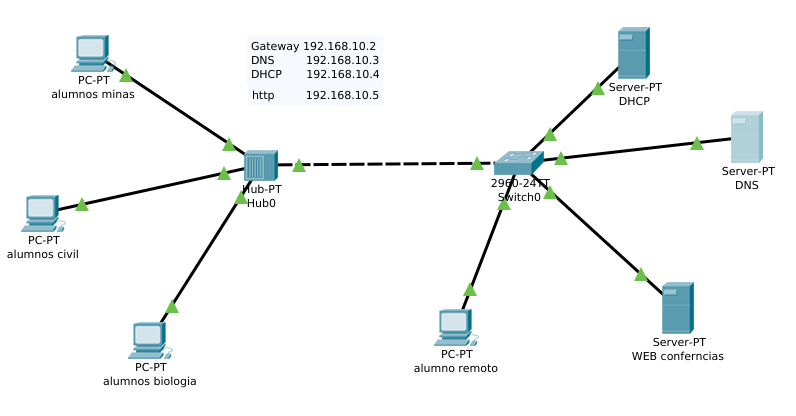
\includegraphics[scale=0.5]{img/confe.png} 
\\ vemos que los alumnos ingresan:\\
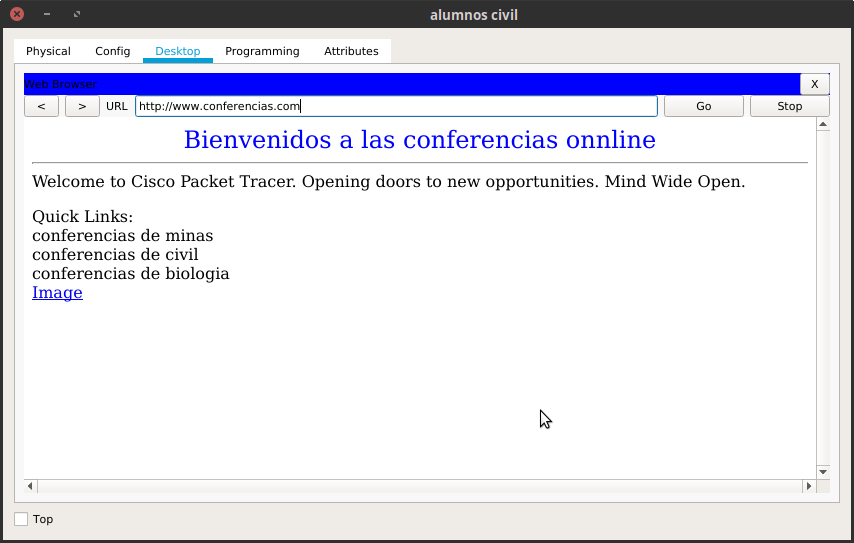
\includegraphics[scale=0.5]{img/civil.png} 
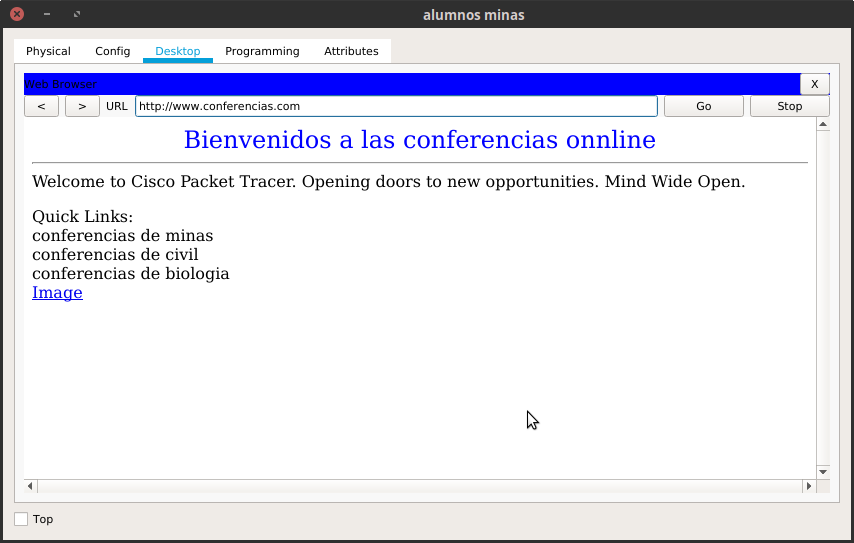
\includegraphics[scale=0.5]{img/minas.png} 
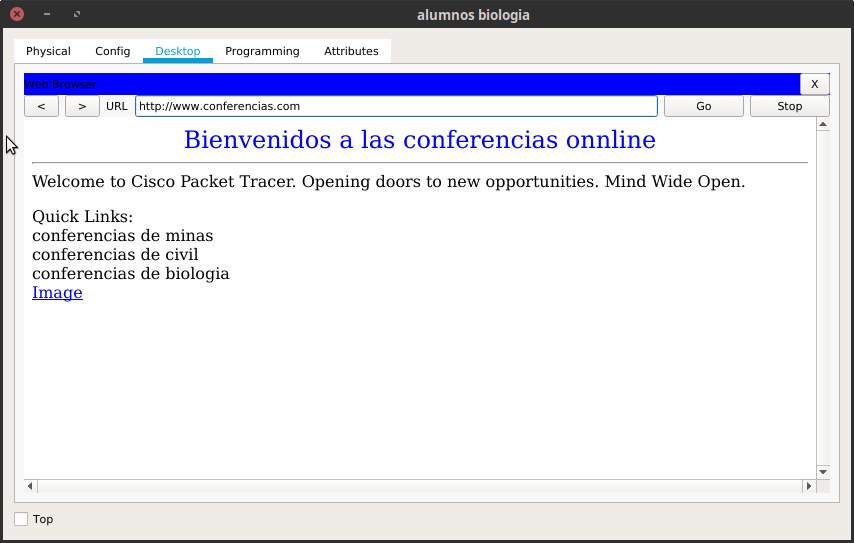
\includegraphics[scale=0.5]{img/biologia.png} 
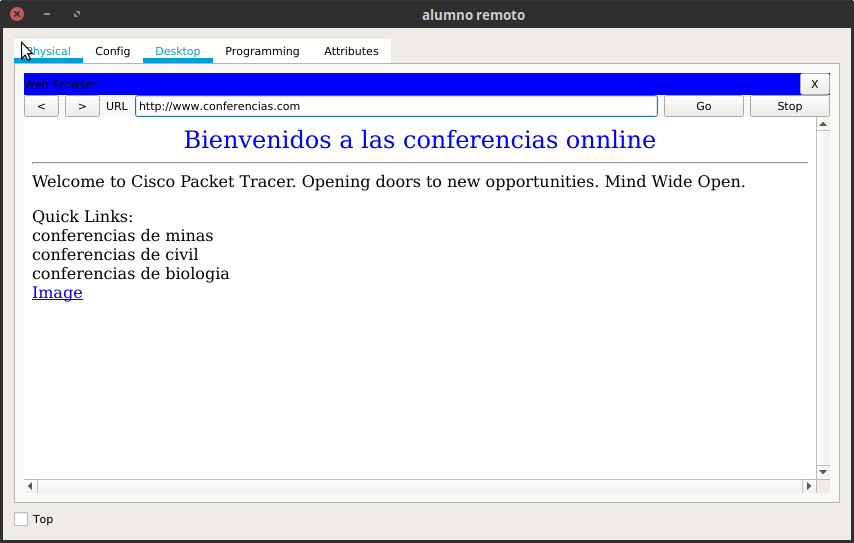
\includegraphics[scale=0.5]{img/otros.png} 
%=========FIN objetivos=========

%procedimiento
%==========================================================
\chapter{CONCLUCIONES}

%=====================================
\section{switch}

\begin{caja}[]{
 Este dispositivo es mucho mas inteligente que el hub. Ademas de existir el switch de capa 3 que ofrece los servicios de un router y switch a la vez. En cisco recomiendan trabajar con switchs de capa 3 para la capa de distribucion, ya que es mucho mas eficiente que un router. Los switchs de capa dos se deben de usar mayormente en capa de acceso en la conexi\'on directa con los pc
 }\end{caja}
 
 \section{Hub}

\begin{caja}[]{
Estos equipos ya pr\'acticamente desaparecieron a causa del switch. su uso ya no se ve actualmente pero se podria recomendra para salas de conferencia en la cual la comunicaci\'on dentro de este ambiente al ser multiple podria ayudar a la comunicaci\'on
 }\end{caja}
 
  \section{laboratorio}

\begin{caja}[]{
El presente laboratorio ayud\'o a establecer las configuraciones iniciales de una lan simple. 
Como vemos la comunicaci\'on es de los computadores que esten conectados al mismo switch y si este switch esta conectado con otro tambi\'en permite la comunicaci\'on esto se debe a que por defecto existe la vlan1 la cual es para todos los puertos.\\
 }\end{caja}
%=========FIN objetivos=========

\end{document}
